\documentclass[10pt,twocolumn]{article}
\usepackage[a4paper,margin=0.72in]{geometry}
\usepackage[T1]{fontenc}
\usepackage[utf8]{inputenc}
\usepackage{times}
\usepackage{graphicx}
\usepackage{booktabs}
\usepackage{array}
\usepackage{multirow}
\usepackage{hyperref}
\usepackage{amsmath}
\usepackage{enumitem}
\usepackage{caption}
\usepackage{subcaption}
\usepackage{float}
\usepackage{xcolor}
\setlength{\columnsep}{0.22in}
\setlength{\parskip}{0.3em}
\setlist[itemize]{leftmargin=*,topsep=2pt,itemsep=1pt,parsep=0pt}
\captionsetup{font=small}
\hypersetup{colorlinks=true, linkcolor=blue, citecolor=blue, urlcolor=blue}
\title{Adaptive Job Search UI Selection with Contextual Bandits:\A Large-Scale Simulated Study}
\author{}
\date{}

\begin{document}

\begin{titlepage}
    \centering
    \vspace*{0.8cm}

    {\Large\scshape National University of Singapore\par}
    \vspace{0.15cm}
    {\large School of Computing\par}

    \vspace{1.0cm}
    \rule{0.82\textwidth}{0.8pt}\par
    \vspace{0.6cm}

    {\Huge\bfseries Adaptive Job-Application UI Selection\par}
    \vspace{0.25cm}
    {\Huge\bfseries with Contextual Bandits\par}

    \vspace{0.7cm}
    \rule{0.82\textwidth}{0.8pt}\par

    \vspace{1.0cm}

    {\Large BT4014 Analytics Driven Design of Adaptive Systems\par}
    \vspace{0.2cm}
    {\Large AY 2025/2026 Semester 2\par}

    \vspace{0.9cm}
    {\LARGE\bfseries Group 7\par}

    \vspace{1.0cm}

    {\large
    \begin{tabular}{c}
    HOVHANNES ANTABLYAN (A0337997B)\\[0.18cm]
    CHANG PAI HUNG (A0339989W)\\[0.18cm]
    ZHANG HAO DONG (A0282115M)\\[0.18cm]
    ABDILLAH SYARIEF SUDRAJAT (A0265840B)
    \end{tabular}\par}

    \vfill

    {\large Submitted for BT4014 Final Project\par}
    \vspace{0.2cm}
    {\large 24 April 2026\par}

\end{titlepage}

\setcounter{page}{1}
\twocolumn[
\maketitle
\begin{abstract}
We study a contextual bandit formulation of adaptive job-platform interface design. The platform must choose one of five application UI variants for each applicant--job interaction, using context features derived from applicant profile, company characteristics, job details, and session intent. Because no suitable real-world dataset was available, we engineer a procedural simulator that generates applicants, companies, jobs, and browsing sessions, then logs approximately 1.05 million interaction outcomes across a full benchmark. Five online policies are evaluated: Epsilon-Greedy, UCB1, Gaussian Thompson Sampling, LinUCB, and Contextual Thompson Sampling. The simulated environment exhibits meaningful heterogeneity by session goal, but the globally strongest UI arm remains \textit{guided\_chat}. As a result, the best overall empirical performer in the final benchmark is Epsilon-Greedy, which rapidly exploits that globally strong arm. The report highlights both the value of contextual modeling and an important design lesson: when the environment contains a dominant global arm, simple exploitation-heavy policies may outperform more sophisticated contextual methods on aggregate reward.
\end{abstract}
\vspace{0.3cm}
]

\section{Introduction}
Modern job platforms expose applicants to many interface designs: ranked lists, card views, swipe-style exploration, or guided assistant flows. These interfaces differ in how much information is surfaced before application, how much reading effort is required, and how effectively they help applicants self-filter. This makes job search an adaptive systems problem: for each applicant-session context, the platform can select a UI that maximizes a downstream reward such as a first-round interview callback.

We formulate this as a contextual bandit problem. Each interaction provides a context vector describing the applicant, job, company, and session. The action is the selected UI arm, and the reward is based on the immediate application outcome, with first-round interview callbacks weighted most heavily and ignored/rejected applications receiving substantially lower value. The report focuses on three questions:
\begin{itemize}
    \item Can procedurally generated job-search contexts produce a realistic large-scale benchmark for adaptive UI selection?
    \item Do contextual bandit algorithms outperform non-contextual baselines in this environment?
    \item What platform-design insights can be extracted from the learned policies and oracle reward landscape?
\end{itemize}

\section{Data and Context}
\subsection{Simulation environment}
The project does not rely on a public real-world hiring dataset. Instead, we generate four linked entities: applicants, companies, jobs, and browsing sessions. The simulator then produces a logged interaction stream in which an applicant views a job through a selected UI arm and may submit an application, be ignored, be rejected, or receive a first-round interview callback.

The environment includes four session goals --- \textit{focused\_search}, \textit{broad\_exploration}, \textit{panic\_apply}, and \textit{casual\_browse} --- and five interface arms:
\begin{itemize}
    \item \textbf{panel\_split}: more detail shown side-by-side for deep inspection,
    \item \textbf{swipe\_fast}: rapid skim / low-friction browsing,
    \item \textbf{card\_grid}: broad comparison across many items,
    \item \textbf{guided\_chat}: assistant-led presentation and recommendation,
    \item \textbf{hybrid\_ranked}: ranked list with intermediate information density.
\end{itemize}

The procedural generator also creates dozens of interpretable signals such as skill match, salary alignment, location alignment, prestige alignment, applicant fatigue, reading patience, decision speed, and self-filter strength. In the exported diagnostic tables, these are combined into a context representation with 48 engineered context features and arm-specific expected reward columns.

\begin{table}[H]
\centering
\caption{Scale of the generated benchmark and evaluation setup.}
\label{tab:setup}
\small
\begin{tabular}{p{0.42\columnwidth}p{0.42\columnwidth}}
\toprule
Component & Value \\
\midrule
UI arms & 5 \\
Session-goal types & 4 \\
Algorithms evaluated & 5 \\
Logged data chunks & 15 parquet chunks \\
Rounds per algorithm & 210{,}000 \\
Total algorithm-rounds & 1.05 million \\
Main reward signal & first-round interview callback \\
\bottomrule
\end{tabular}
\end{table}

\subsection{Why simulation is appropriate}
The project guidelines explicitly allow simulation when real-world data are unavailable, provided the data construction process is clearly explained. Here, simulation is useful because the central objective is not historical prediction; it is controlled evaluation of adaptive interface policies under varying user needs and browsing styles. The simulator lets us encode plausible trade-offs between information richness, dwell time, fatigue accumulation, and application quality while still producing a benchmark large enough for online learning and regret analysis.

\section{Methods}
We evaluate five online policies:
\begin{itemize}
    \item \textbf{Epsilon-Greedy}: simple explore/exploit baseline.
    \item \textbf{UCB1}: optimism-based non-contextual baseline.
    \item \textbf{Gaussian Thompson Sampling}: non-contextual Bayesian baseline.
    \item \textbf{LinUCB}: contextual linear upper-confidence method.
    \item \textbf{Contextual Thompson Sampling}: contextual Bayesian linear method.
\end{itemize}

At each round, the simulator first produces the applicant--job--session context. The policy chooses a UI arm, the world model computes the chosen arm's expected reward, and then a realized outcome is sampled. We log both realized reward and instantaneous expected regret relative to the oracle arm for that exact context. This gives us two complementary evaluation views: cumulative realized performance and regret with respect to the best available action.

In addition to algorithm evaluation, the pipeline exports summary tables and figures for interpretability. These include a reward-landscape heatmap by session goal and arm, cumulative contextual regret, rolling realized reward, arm-selection frequencies, outcome mixes, and lightweight summary tables for final reporting.

\section{Experimental Results}
\subsection{Oracle reward landscape}
Figure~\ref{fig:landscape} shows that the simulator does contain meaningful context dependence. The row-wise best arm differs by session goal: \textit{panel\_split} is strongest for \textit{focused\_search}, \textit{card\_grid} is strongest for \textit{broad\_exploration}, \textit{swipe\_fast} is strongest for \textit{panic\_apply}, and \textit{hybrid\_ranked} is strongest for \textit{casual\_browse}. This confirms that the task is a reasonable contextual decision problem rather than a trivial constant-policy benchmark.

At the same time, the global per-arm expected rewards averaged over the whole environment remain relatively close, with \textit{guided\_chat} having the strongest global average expected reward (approximately 0.173), followed by \textit{hybrid\_ranked} (0.169) and \textit{panel\_split} (0.167). This gap is important for interpreting the final winner.

\begin{figure*}[t]
    \centering
    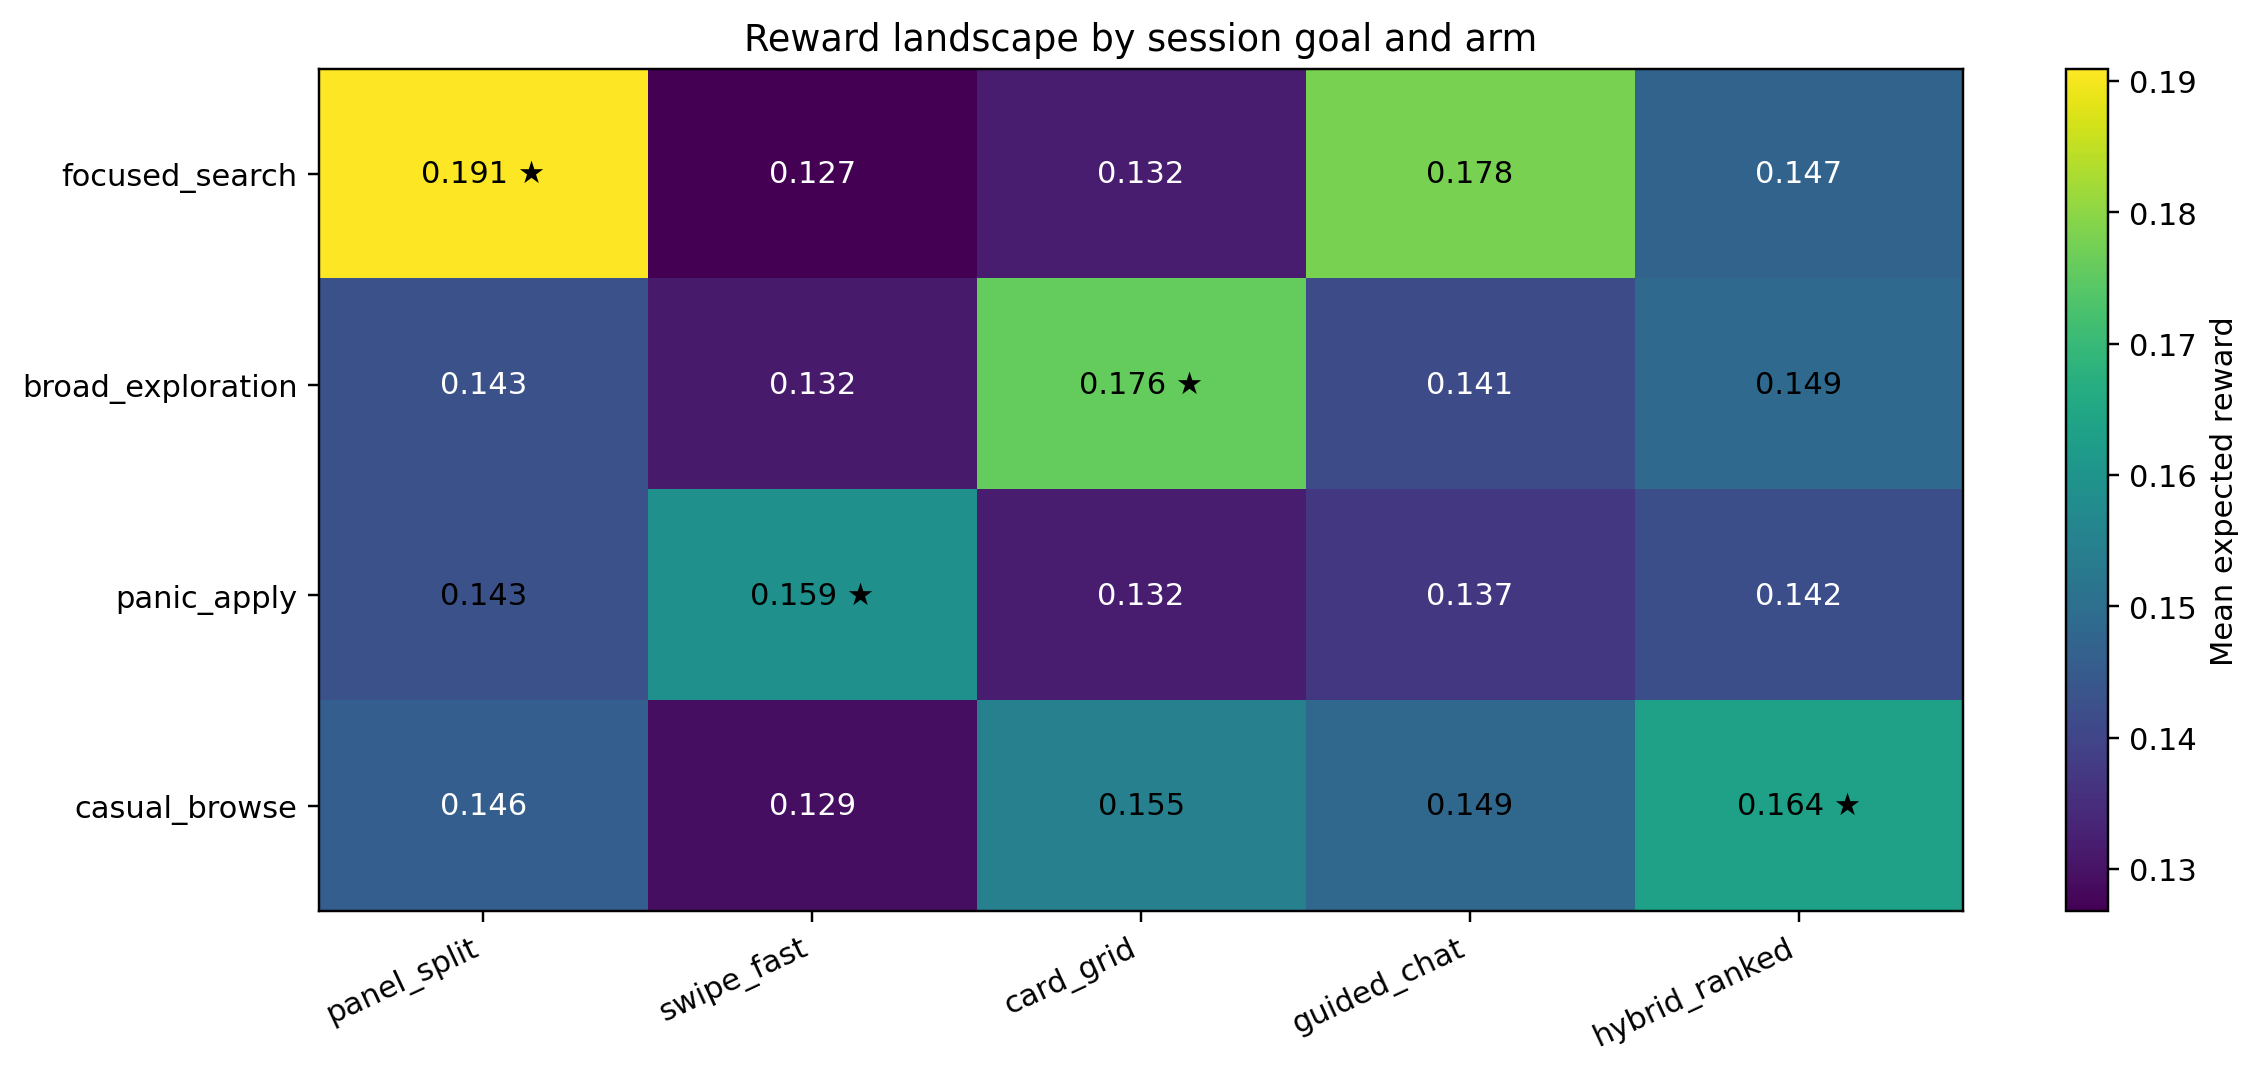
\includegraphics[width=0.88\textwidth]{reward_landscape_heatmap.png}
    \caption{Mean expected reward by session goal and UI arm. A star marks the best arm within each session-goal row. The simulator is heterogeneous: no single arm dominates every row.}
    \label{fig:landscape}
\end{figure*}

\subsection{Algorithm ranking}
Table~\ref{tab:algos} summarizes the final benchmark. Somewhat counter to the original expectation that contextual methods would dominate, the strongest aggregate performer is \textbf{Epsilon-Greedy}. It achieves the highest final cumulative reward (31,232.5) and the lowest cumulative expected regret (294.3). Gaussian Thompson Sampling is second, while LinUCB and Contextual Thompson Sampling trail slightly behind.

\begin{table*}[t]
\centering
\caption{Final online evaluation summary over 210,000 rounds per algorithm. Interview rate and ignore rate are percentages of all rounds.}
\label{tab:algos}
\small
\begin{tabular}{lrrrrr}
\toprule
Algorithm & Final cumulative reward & Final cumulative regret & Mean reward & Interview rate (\%) & Ignore rate (\%) \\
\midrule
Epsilon-Greedy & 31,232.5 & 294.3 & 0.1487 & 15.40 & 56.60 \\
Gaussian TS & 30,971.4 & 758.1 & 0.1475 & 15.04 & 56.88 \\
LinUCB & 30,812.4 & 1,047.6 & 0.1467 & 14.74 & 57.61 \\
Contextual TS & 30,731.7 & 1,072.7 & 0.1463 & 14.66 & 57.70 \\
UCB1 & 30,707.8 & 1,485.9 & 0.1462 & 14.61 & 57.74 \\
\bottomrule
\end{tabular}
\end{table*}

Figure~\ref{fig:regret} visualizes the same result over time. Epsilon-Greedy remains the lowest-regret curve throughout most of the run, and UCB1 is consistently the worst. The ranking is stable enough that the result does not appear to be a late-run fluctuation.

\begin{figure*}[t]
    \centering
    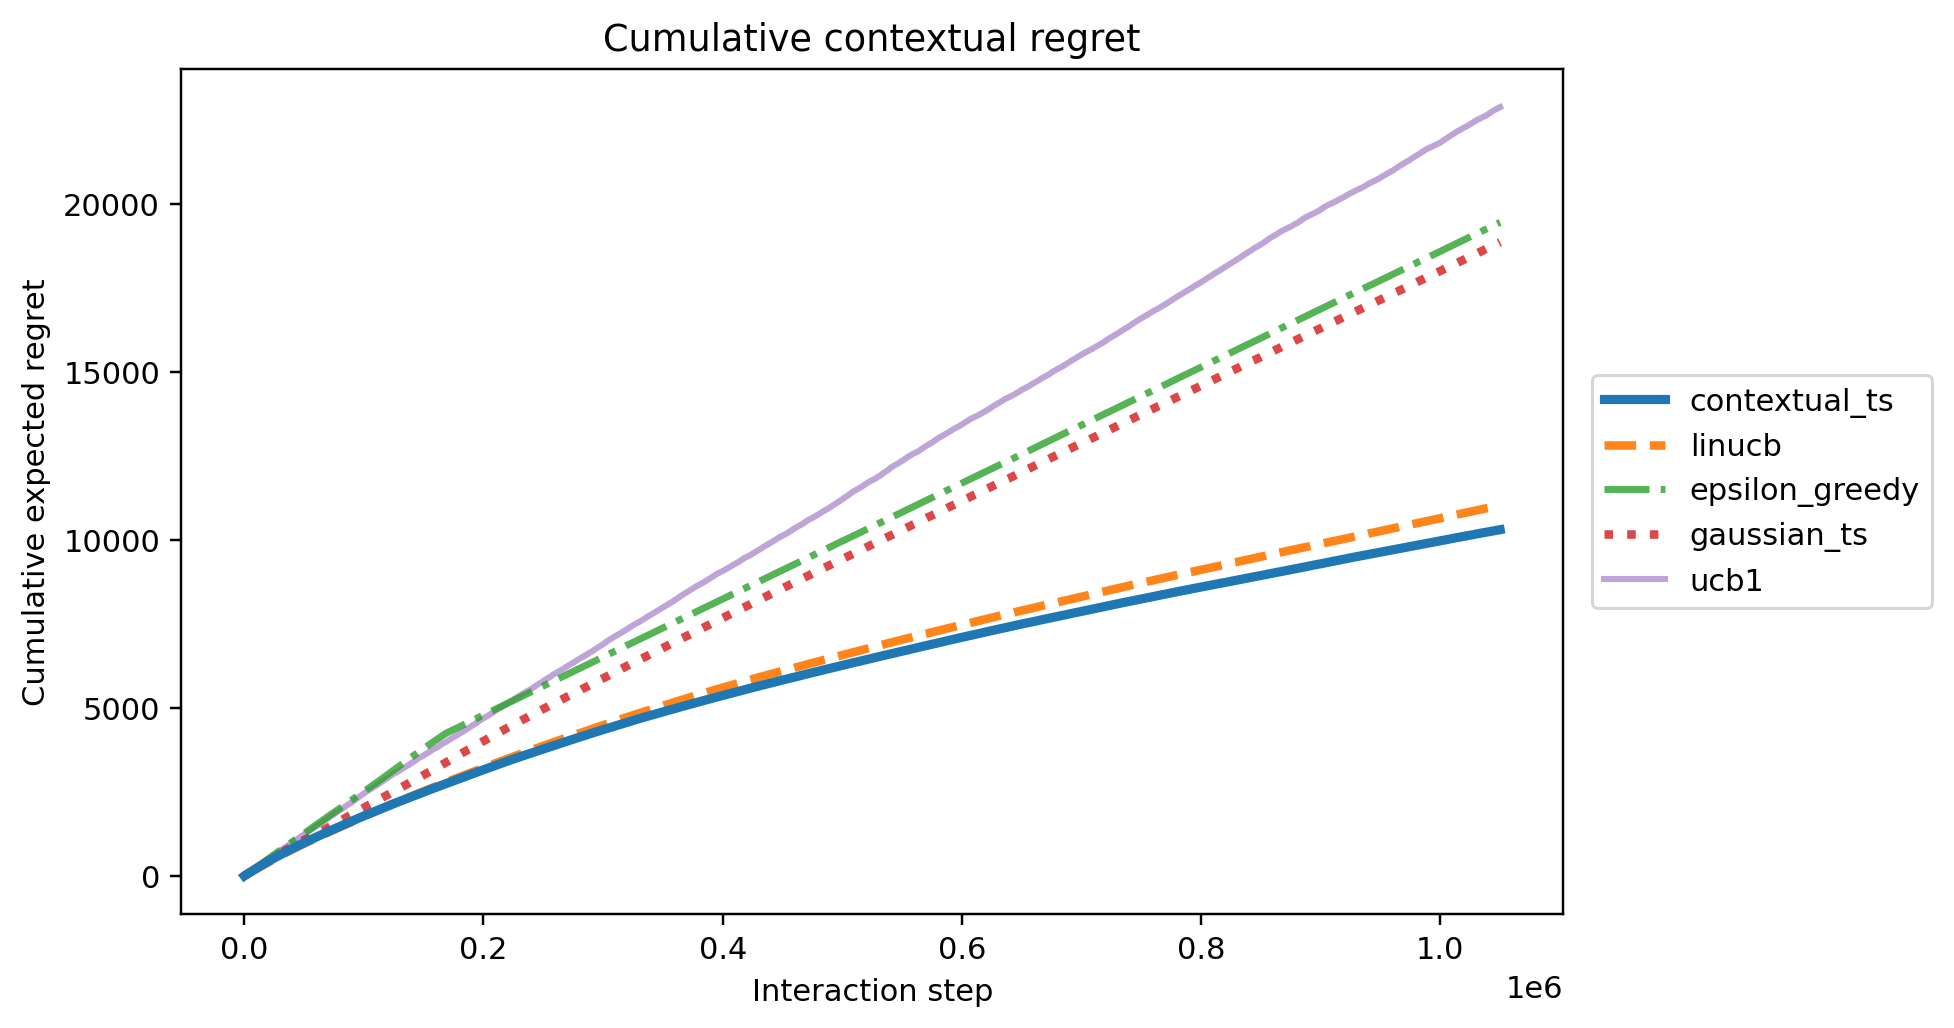
\includegraphics[width=0.86\textwidth]{cumulative_contextual_regret.png}
    \caption{Cumulative expected regret over the full benchmark. Lower is better. Epsilon-Greedy achieves the smallest total regret, while UCB1 is consistently worst.}
    \label{fig:regret}
\end{figure*}

\subsection{Why did Epsilon-Greedy win?}
Figure~\ref{fig:behaviour} helps explain the result. Epsilon-Greedy selects \textit{guided\_chat} in about 95.7\% of rounds, effectively collapsing to a near-constant policy. In this simulator, that turns out to be highly competitive because \textit{guided\_chat} has the highest global average expected reward even though it is not the best arm in every session-goal row. Contextual methods allocate traffic more broadly and therefore capture more of the row-specific structure, but they also pay a price for exploration and model mismatch.

This is an important systems insight rather than a failure of the contextual formulation. In environments where one arm is globally strong and context advantages are modest, aggressive exploitation can outperform more sophisticated contextual learning in total reward. A platform designer should therefore not assume that ``more advanced'' policies automatically produce better outcomes; the reward landscape itself determines whether contextual complexity is worthwhile.

\begin{figure*}[t]
\centering
% Set a width for the subfigure box, but limit the internal image height
\begin{subfigure}[t]{\textwidth}
    \centering
    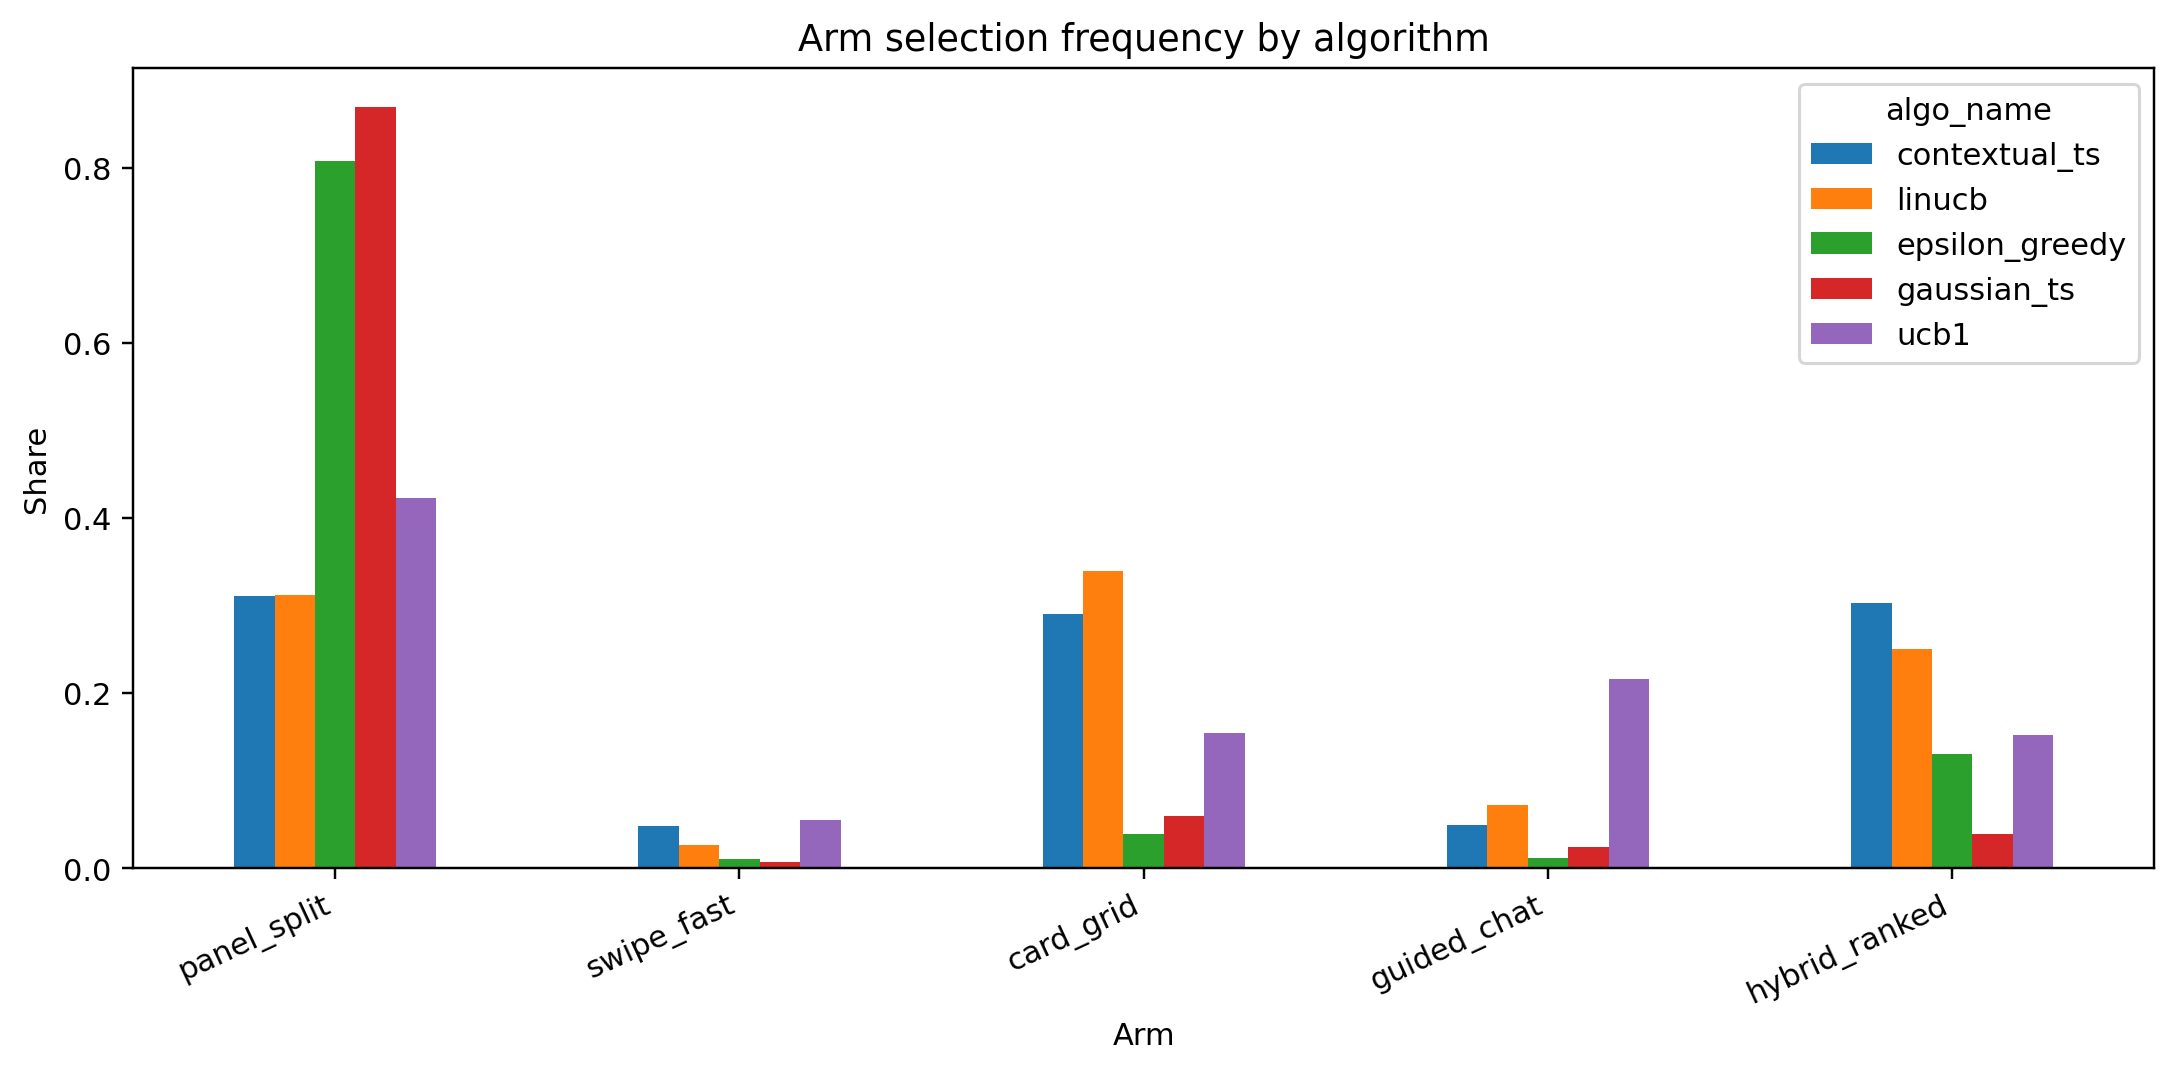
\includegraphics[width=0.8\textwidth, height=0.35\textheight, keepaspectratio]{arm_selection_frequency.png}
    \caption{Arm-selection frequency by algorithm.}
\end{subfigure}

\vspace{1em} % Small buffer space

\begin{subfigure}[t]{\textwidth}
    \centering
    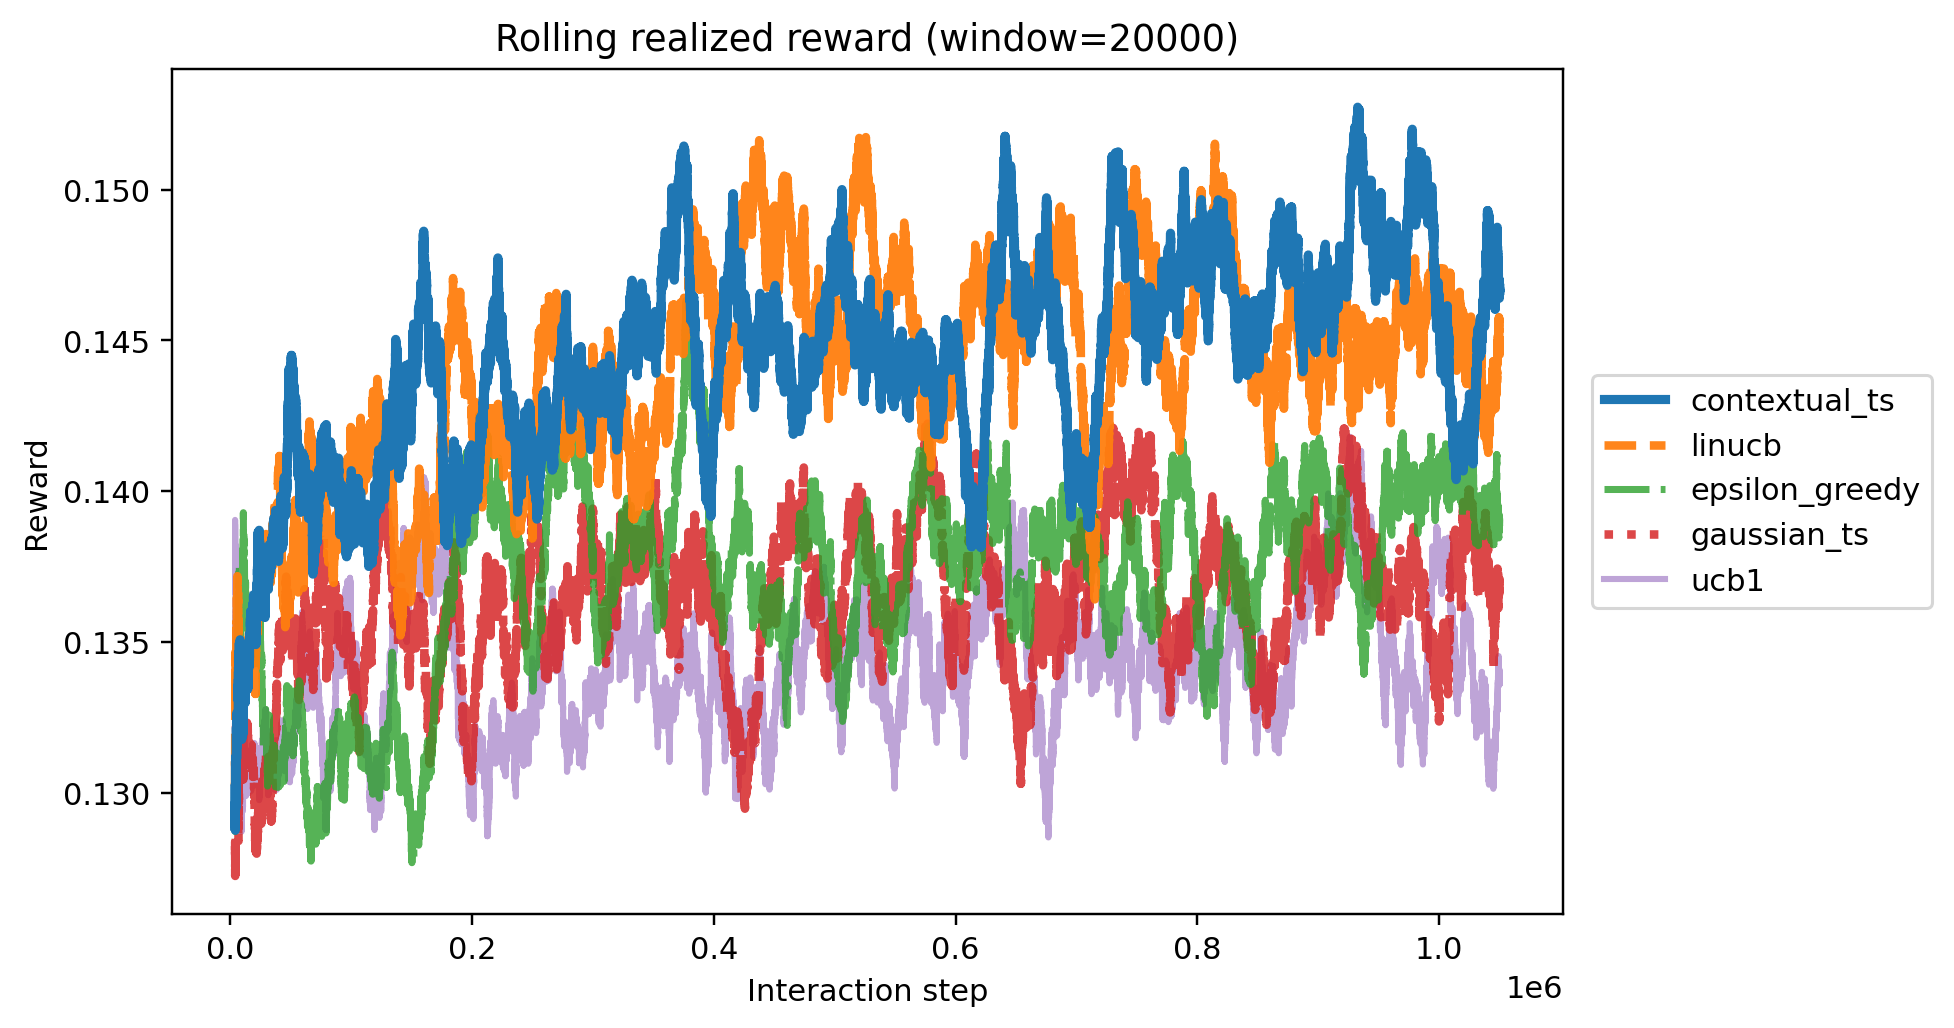
\includegraphics[width=0.8\textwidth, height=0.35\textheight, keepaspectratio]{rolling_avg_reward.png}
    \caption{Rolling realized reward.}
\end{subfigure}
\caption{Behavioral interpretation of the benchmark. Epsilon-Greedy wins partly because it quickly concentrates on the globally strongest arm, while contextual methods distribute traffic more widely.}
\label{fig:behaviour}
\end{figure*}


\section{Discussion and Limitations}
The project demonstrates that a procedurally generated benchmark can support meaningful contextual bandit analysis for adaptive interface design. The environment clearly differentiates applicant needs and session goals, and the learned arm-selection patterns are interpretable. The exported pipeline also scales to large offline artifacts, including raw tables, logged chunks, processed parquet files, and figure-ready summaries.

However, several limitations remain. First, the environment is still simulated and therefore only as realistic as its generative assumptions. Second, the reward is intentionally narrow: we stop at the first-round interview stage and do not model later funnel steps such as offers or long-term retention. Third, the contextual algorithms rely on relatively simple linear structure; richer nonlinear policies or representation learning could behave differently. Finally, the current benchmark suggests that the context signal is present but not strong enough to overcome the advantage of a globally dominant arm. A stronger heterogeneity design or more sharply differentiated arm profiles could change the ranking.

\section{Conclusion}
We presented a contextual bandit benchmark for adaptive job-search UI selection and evaluated five online policies on a large simulated interaction stream. The simulator creates applicant, job, company, and session contexts and uses them to model how different interface designs affect self-filtering, information comprehension, fatigue, and first-round interview outcomes.

The most important empirical result is that \textbf{Epsilon-Greedy performs best overall} in the final benchmark, despite the contextual nature of the task. This happens because \textit{guided\_chat} is globally very strong, so a fast-exploiting policy captures most of the available value. Nevertheless, the oracle reward landscape still shows that the best interface depends on session goal, which validates the contextual framing and highlights where more nuanced policies may matter.

For platform design, the takeaway is practical: adaptive UI optimization should be driven by measured reward structure, not only by algorithmic sophistication. If one interface is globally robust, simple policies may already capture most of the gain. If user intent segments become more sharply differentiated, contextual policies become more attractive.

\paragraph{AI use acknowledgement.} We used ChatGPT as a coding and writing assistant during this project. Specifically, it was used to help review repository organization, refine notebook/report structure, debug packaging and Git commands, and draft/edit parts of the README, presentation transcript, and report wording. Representative prompts included requests to organize files for submission, explain bandit plots in plain language, and convert our outputs into a concise scientific-style report. 

\begin{thebibliography}{9}
\bibitem{bouneffouf2020}
Bouneffouf, D., Rish, I., Aggarwal, C.: Survey on applications of multi-armed and contextual bandits. In: \emph{2020 IEEE Congress on Evolutionary Computation}, pp. 1--8 (2020)

\bibitem{li2010}
Li, L., Chu, W., Langford, J., Schapire, R.: A contextual-bandit approach to personalized news article recommendation. In: \emph{Proceedings of WWW}, pp. 661--670 (2010)

\bibitem{agrawal2013}
Agrawal, S., Goyal, N.: Thompson sampling for contextual bandits with linear payoffs. In: \emph{Proceedings of ICML}, pp. 127--135 (2013)

\bibitem{guidelines}
BT4014 Final Project Guidelines, AY2025/2026 Semester 2. Project description, submission requirements, and AI-use policy.\hfill
\end{thebibliography}

\end{document}
